
\section{Results and Discussion}
\label{sec:results}

\subsection{Campaign Validity}

All 432 runs completed and are used; each of the 144 context--policy cells contains three
paired replications, and the measured cohort ranges from 361--392 vehicles per run at
720\,veh/h to 862--906 at 1680\,veh/h, totalling 270{,}432 trips.

One property of the campaign shapes everything that follows. Insertion delay --- time
spent waiting to enter the network --- is negligible at 720\,veh/h (0.12\,s averaged over
all 432 runs), small at 1200\,veh/h (5.54\,s) and large at 1680\,veh/h (262.41\,s, with
810.29\,s in the worst single run), and it is strongly policy-dependent: at 1680\,veh/h it
averages 447.5\,s under SP against 6.3\,s under DTT. The highest demand level therefore
operates at the edge of what the network can accept, and absolute journey times there
partly describe the insertion queue rather than in-network travel.
Section~\ref{sec:robust} shows that the policy \emph{ordering} does not depend on this
boundary; the absolute values clearly do.

\subsection{Regime-Dependent Policy Preference}

Define the switching margin between the two unconstrained policies as
\begin{equation}
m_s = C_{s,\mathrm{SP}} - C_{s,\mathrm{DTT}},
\label{eq:margin}
\end{equation}
so a negative value means SP has the lower observed cost. Fig.~\ref{fig:performance}
shows the physical outcomes, Fig.~\ref{fig:regime} the resulting structure and
Table~\ref{tab:margin} the values.

\begin{figure}[tb]
\centering
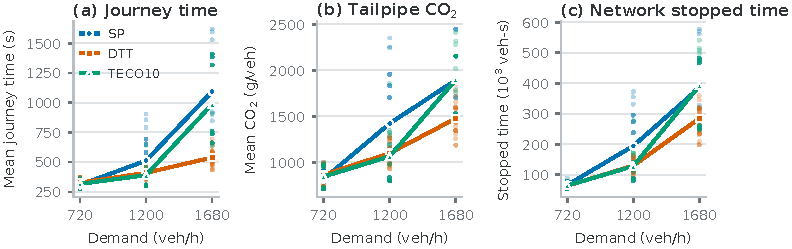
\includegraphics[width=\linewidth]{figures/fig2_performance.pdf}
\caption{Policy outcomes against demand. Lines are means over the eight contexts at
each demand level; faint points are individual runs. The three panels separate the two
primary criteria from the system-level congestion diagnostic. The policies are
near-indistinguishable at 720\,veh/h and separate sharply above it.}
\label{fig:performance}
\end{figure}

\begin{figure}[tb]
\centering
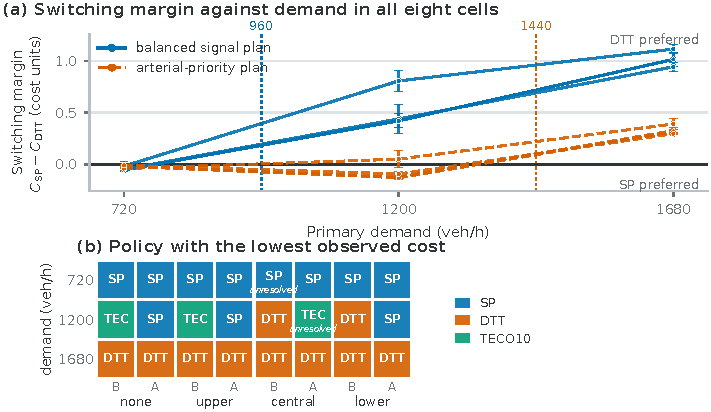
\includegraphics[width=\linewidth]{figures/fig3_regime.pdf}
\caption{(a) The switching margin of Eq.~\eqref{eq:margin} in all eight
restriction--signal cells; error bars are $\pm2$ standard errors over three paired seeds
and are descriptive, not a significance test. Dotted lines mark the two demand
thresholds fitted by the selection rules of Section~\ref{sec:selection}. (b) The policy
with the lowest observed cost in each context; the two contexts whose margin is not
resolved against replication dispersion are marked.}
\label{fig:regime}
\end{figure}

\begin{table}[htb]
\centering\footnotesize
\caption{Switching margin $m_s$ with its standard error over three paired seeds.
Negative values favour SP. The bracket is the interval of the tested demand grid in
which the sign changes; it is not a threshold estimate. $\dagger$ marks the two contexts
where $|m_s|\le 2\,\mathrm{SE}$.}
\label{tab:margin}
\setlength{\tabcolsep}{2.9pt}
\begin{tabular}{@{}llrrrrrrl@{}}
\toprule
& & \multicolumn{2}{c}{720\,veh/h} & \multicolumn{2}{c}{1200\,veh/h}
& \multicolumn{2}{c}{1680\,veh/h} & \\
\cmidrule(lr){3-4}\cmidrule(lr){5-6}\cmidrule(lr){7-8}
Signal & Restr. & $m_s$ & SE & $m_s$ & SE & $m_s$ & SE & Bracket\\
\midrule
Bal & none & $-0.0551$ & 0.0064 & $+0.4204$ & 0.0334 & $+1.0139$ & 0.0323 & (720,\,1200]\\
Bal & upper & $-0.0515$ & 0.0071 & $+0.4382$ & 0.0697 & $+0.9418$ & 0.0232 & (720,\,1200]\\
Bal & central & $-0.0195$ & 0.0220$^{\dagger}$ & $+0.8056$ & 0.0502 & $+1.1137$ & 0.0233 & (720,\,1200]\\
Bal & lower & $-0.0562$ & 0.0058 & $+0.4196$ & 0.0334 & $+1.0134$ & 0.0323 & (720,\,1200]\\
\midrule
Art & none & $-0.0184$ & 0.0046 & $-0.1269$ & 0.0101 & $+0.3249$ & 0.0162 & (1200,\,1680]\\
Art & upper & $-0.0198$ & 0.0057 & $-0.1318$ & 0.0019 & $+0.3165$ & 0.0112 & (1200,\,1680]\\
Art & central & $-0.0423$ & 0.0015 & $+0.0488$ & 0.0423$^{\dagger}$ & $+0.3893$ & 0.0250 & (720,\,1200]\\
Art & lower & $-0.0110$ & 0.0054 & $-0.0954$ & 0.0129 & $+0.2952$ & 0.0052 & (1200,\,1680]\\
\bottomrule
\end{tabular}
\end{table}

The structure is systematic rather than confined to one configuration: at 720\,veh/h the
margin is negative in all eight cells and at 1680\,veh/h positive in all eight. Over the
full portfolio, SP has the lowest observed cost in all eight low-demand contexts and DTT
in all eight high-demand contexts, while the intermediate level splits three ways --- SP
in three contexts, TECO10 in three and DTT in two. All three portfolio members win
somewhere, which establishes complementarity in the sense of Section~3.3; what that is
worth is a separate question (Section~\ref{sec:value}).

The signal plan displaces the crossing. Under balanced timing the margin has already
changed sign by 1200\,veh/h in all four restriction configurations; under
arterial-priority timing it is still negative at 1200\,veh/h in three of four and changes
sign only by 1680\,veh/h. The mean margin at 1200\,veh/h is $+0.5209$ under balanced
timing against $-0.0763$ under arterial priority, a difference of $0.5972$ cost units, so
the displacement is at least one full step of the grid, 480\,veh/h; the grid cannot say
how much more. The approach is also not uniform: under balanced timing the margin
increases with demand in all four cells, whereas under arterial priority it
\emph{decreases} from 720 to 1200\,veh/h in three of four cells before rising sharply.
Restriction location moves the margin very little --- the four balanced cells at
1200\,veh/h span $+0.4196$ to $+0.8056$, three of them within $0.02$ of each other ---
which foreshadows the feature ablation of Section~\ref{sec:selection}.

\subsection{Resolution of the Switching Boundary}
\label{sec:noise}

The experiment brackets the sign change but does not locate it
(Section~\ref{sec:boundary-exp}). What the completed data establish is that the brackets
rest on margins large relative to replication dispersion: 22 of the 24 margins in
Table~\ref{tab:margin} satisfy $|m_s|>2\,\mathrm{SE}(m_s)$, the smallest ratio among
those being 2.03. The two exceptions are the balanced central-restriction context at
720\,veh/h ($m=-0.0195$, $\mathrm{SE}=0.0220$) and the arterial central-restriction
context at 1200\,veh/h ($m=+0.0488$, $\mathrm{SE}=0.0423$). These are exactly the two
contexts in which the sign of the margin differs across the three seeds, so the
descriptive criterion and the direct seed-by-seed check agree. This also explains the one
cell that breaks the signal-plan pattern: the arterial central cell is assigned the
$(720,1200]$ bracket on the strength of a margin whose sign three replications do not
agree on, so seven of the eight cells have a resolved bracket and the eighth does not.

Dispersion is not uniform: the standard error of the margin has a median of 0.0057 cost
units at 720\,veh/h, 0.0334 at 1200\,veh/h and 0.0232 at 1680\,veh/h, with its maximum,
0.0697, also at 1200\,veh/h. Replication noise is largest precisely in the band where the
ordering changes --- the band in which a decision is hardest and, as the next subsection
shows, the one carrying most of the available decision value.

\subsection{Decision Value of Adaptation}
\label{sec:value}

Complementarity is established, but its value is modest. Over the 24 contexts the single
best fixed policy is DTT, with mean decision regret 0.03018 cost units; fixed SP and
fixed TECO10 cost 0.31825 and 0.20757. Under leave-one-context-out the depth-3 selector
attains mean regret 0.00606, chooses the lowest-cost policy in 21 of 24 contexts and is
within 1\,\% of the context optimum in 22 of 24, so by Eq.~\eqref{eq:headroom} it captures
$G=(0.03018-0.00606)/0.03018=0.799$: 79.9\,\% of the available decision headroom.

This percentage is a decision statistic and nothing else. It is \emph{not} a 79.9\,\%
reduction in travel time, emissions or any physical quantity. In physical terms the
selected policies average 412.17\,s and 1114.64\,g per vehicle against 425.17\,s and
1145.36\,g under fixed DTT --- 13.00\,s (3.06\,\%) and 30.71\,g (2.68\,\%) lower over the
evaluated contexts, with a hindsight bound of 409.25\,s and 1106.12\,g. The decision
statistic says how much of the attainable improvement was realised; the physical figures
say how large the attainable improvement was.

The headroom is highly localised (Fig.~\ref{fig:decision}b). At 1680\,veh/h DTT is best
in all eight contexts, so there is nothing for adaptation to win: the fixed policy has
exactly zero mean regret and the entire penalty in that regime belongs to choosing the
\emph{wrong} fixed policy, which costs 0.67611 under SP. At 720\,veh/h the fixed policy
carries 0.03422 and the selector removes all of it; the transition band carries 0.05633,
of which the selector removes about two thirds, leaving 0.01818. Weighted by the eight
contexts in each regime, 37.8\,\% of the total headroom sits at low demand, 62.2\,\% in
the transition band and none at high demand.

Two conclusions follow and they point in different directions. Adaptation is worth having,
but it is worth much less than choosing the right fixed policy: the difference in mean
regret between the best and worst fixed policy, 0.28807 cost units, is nearly ten times
the entire headroom adaptation competes for. The first-order operational result is about
the fixed choice; adaptation is a second-order refinement concentrated in one demand
band.

\subsection{Noise and Effect Size}

A headroom of 0.03018 should be checked against the dispersion of the benchmark that
produced it. Recomputing the whole decision analysis independently within each seed block
gives 0.04138, 0.03035 and 0.02959 cost units, a mean of 0.03377 with a standard error of
0.00381 across blocks. The quantity the selector competes for is therefore roughly eight
times the dispersion of its own estimate --- enough for the comparison above to be
meaningful, but not enough to treat its fifth decimal place as stable; the differences
that matter are the order-of-magnitude ones, 0.318 against 0.030 against 0.006. At context
level the picture is less reassuring in the transition band, where the median absolute
margin is 0.2757 cost units against a median standard error of 0.0334 but individual
ratios run down to the two unresolved contexts above, and all three of the selector's
remaining errors fall in that band. The difficulty is concentrated where the data are
noisiest --- expected for a boundary-detection task, and the main reason the residual
20\,\% of the headroom is not recovered.
